\usetikzlibrary{matrix}
\usetikzlibrary{arrows,shapes}
\usetikzlibrary{positioning,er}
\usetikzlibrary{decorations}

\newcommand{\bomverse}{
	\node[text height=1em, text width=1em]{};}

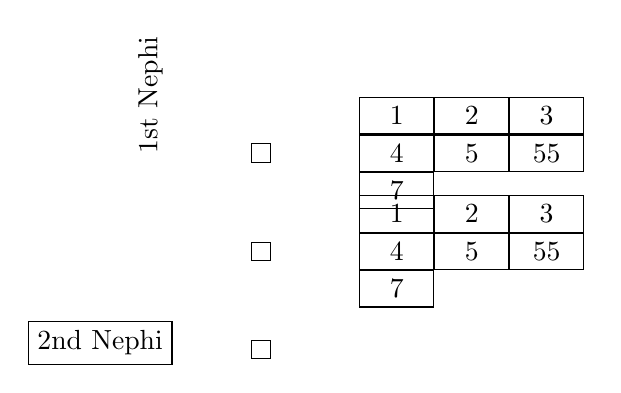
\begin{tikzpicture}%[every node/.style={
	%text height=1em,
	%text width=1em
	%}]
\node [anchor=center, ](Ne1){\rotatebox{90}{1st Nephi}};
\node [base right=of Ne1, draw](Ne1list){};
%\node [anchor=northeast](Ne1list2){list2};
\begin{scope}[every node/.style={text width=2em, align=flush center}]
\matrix [right=of Ne1list,matrix of math nodes,nodes={draw}]
{
1 & 2 & 3 \\
 4 & 5  & 55 \\
 7&  & \\
};
\end{scope}
\node[anchor = base, below=of Ne1list, draw](Ne1list2){};

\begin{scope}[every node/.style={text width=2em, align=flush center}]
\matrix [right=of Ne1list2,matrix of math nodes,nodes={draw}]
{
1 & 2 & 3 \\
 4 & 5  & 55 \\
 7&  & \\
};
\end{scope}




\node[anchor = base, below=of Ne1list2, draw](Ne2list){};

\node[base left=of Ne2list, draw]{2nd Nephi};




\end{tikzpicture}